\documentclass{article}

\usepackage{geometry}
\geometry{letterpaper, margin=2cm}
\usepackage{amsmath}
\usepackage{graphicx}
\usepackage{subfigure}

\usepackage[section]{placeins}
\let\Oldsection\section
\renewcommand{\section}{\FloatBarrier\Oldsection}
\let\Oldsubsection\subsection
\renewcommand{\subsection}{\FloatBarrier\Oldsubsection}
\let\Oldsubsubsection\subsubsection
\renewcommand{\subsubsection}{\FloatBarrier\Oldsubsubsection}

\title{Structures Report}
\author{Reinaldo Zapata}
\date{}

\pagestyle{empty}
\thispagestyle{empty}

\begin{document}
\maketitle

%%%%%%%%%%%%%%%%%%%%%%%%%%%%%%%%%%%%%%%%%%%%%%%%%%%%%%%%%%%%%%%%%%%%%%%%%%%%%%%%
%%%%%%%%%%%%%%%%%%%%%%%%%%%%%%%%%%% UP %%%%%%%%%%%%%%%%%%%%%%%%%%%%%%%%%%%%%%%%%
%%%%%%%%%%%%%%%%%%%%%%%%%%%%%%%%%%%%%%%%%%%%%%%%%%%%%%%%%%%%%%%%%%%%%%%%%%%%%%%%

\section{Up} % (fold)
\label{sec:up}

%%%%%%%%%%%%%%%%%%%%%%%%%%%%% xb [0.0:0.2] %%%%%%%%%%%%%%%%%%%%%%%%%%%%%%%%%%%%%

\subsection{$\mathcal{V}^{\mathrm{xb}} $: energy range: 0.0--0.2 eV }
\begin{figure}[h]
    \centering
    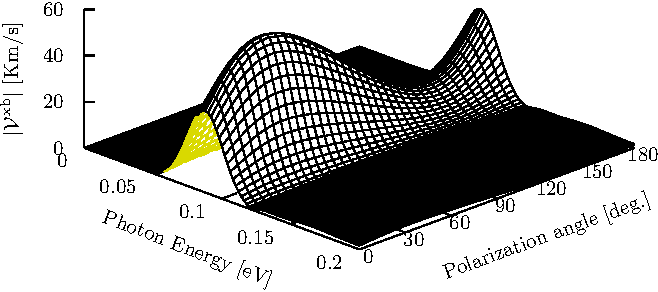
\includegraphics[width=0.7\textwidth]{upplots/up-magvxb-incang-1-4545.pdf}
    \caption{The most intense response for $\mathcal{V}^{\mathrm{xb}} $ is for 
    40$^{\circ}$.}
    \label{fig:up-magvxbincang1}
\end{figure}
\begin{figure}[h]
    \centering
    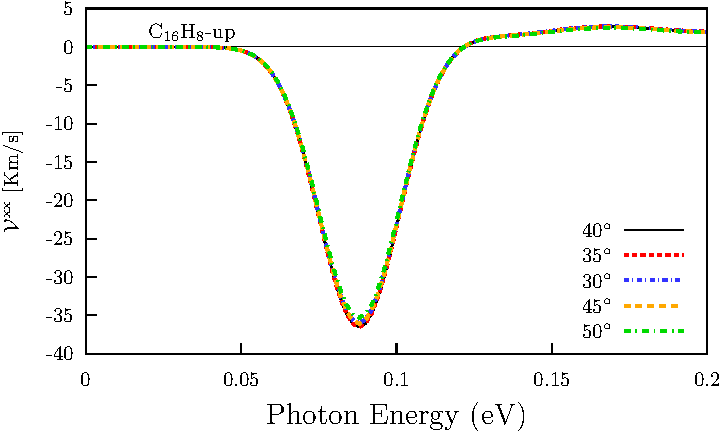
\includegraphics[width=0.45\textwidth]{upplots/up-vab-xx-angcomp.pdf}
    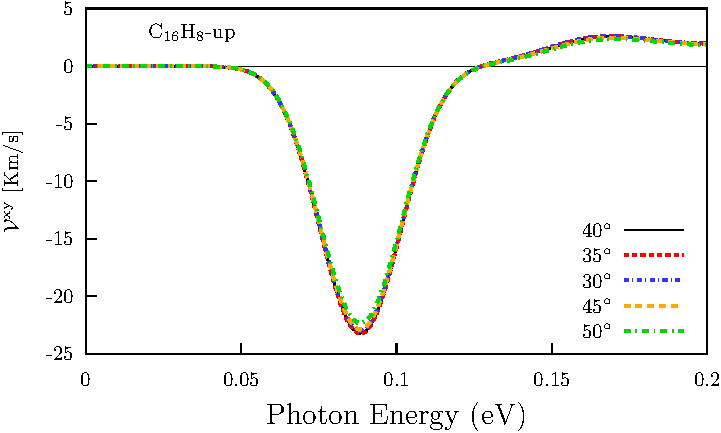
\includegraphics[width=0.45\textwidth]{upplots/up-vab-xy-angcomp.pdf}\\
    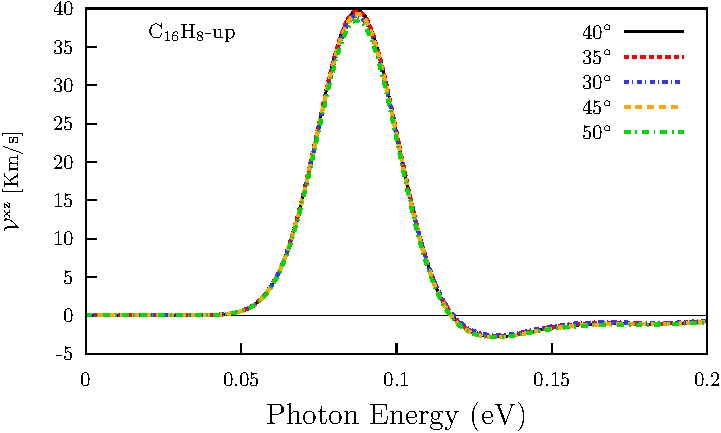
\includegraphics[width=0.45\textwidth]{upplots/up-vab-xz-angcomp.pdf}
    \caption{Cheking angle of incidence for $xb$ components for up structure.}
    \label{fig:up-xbangcomp}
\end{figure}
\begin{figure}[tb]
    \centering
    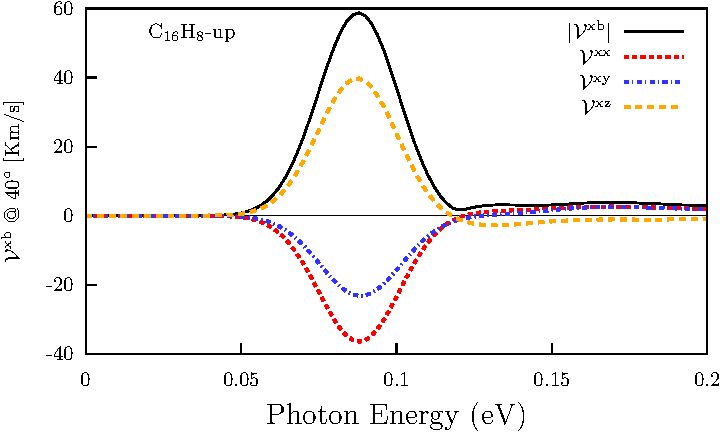
\includegraphics[width=0.7\textwidth]{upplots/up-vab-xb-1.pdf}
    \caption{Three components of $\mathcal{V}^{\mathrm{xb}} $ @ 40$^{\circ}$.}
    \label{fig:up-vxb1}
\end{figure}



%%%%%%%%%%%%%%%%%%%%%%%%%%%%% yb [0.0:0.2] %%%%%%%%%%%%%%%%%%%%%%%%%%%%%%%%%%%%%

\subsection{$\mathcal{V}^{\mathrm{yb}} $: energy range: 0.0--0.2 eV }
\begin{figure}[h]
    \centering
    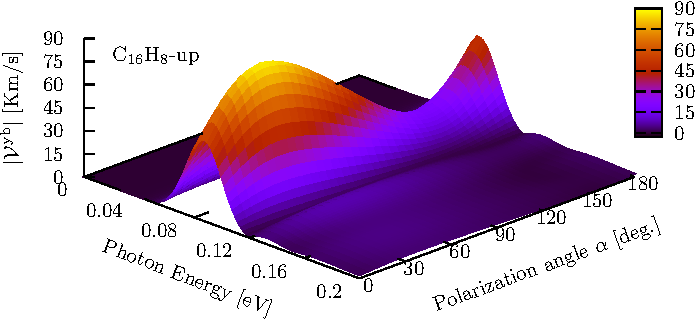
\includegraphics[width=0.7\textwidth]{upplots/up-magvyb-incang-1-4545.pdf}
    \caption{The most intense response for $\mathcal{V}^{\mathrm{yb}} $ is for 
    40$^{\circ}$.}
    \label{fig:up-magvybincang1}
\end{figure}
\begin{figure}[ht]
    \centering
    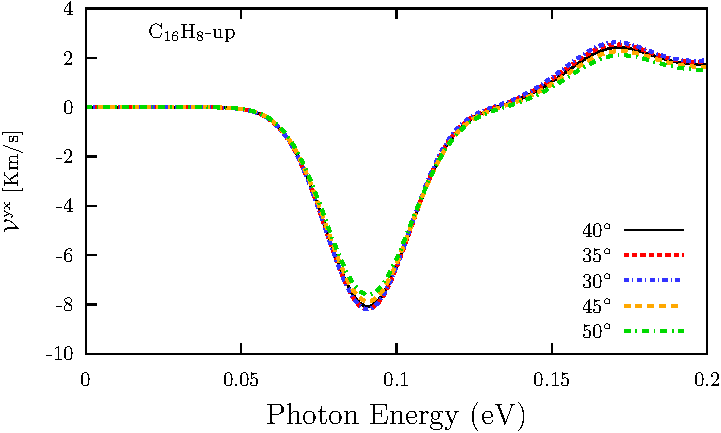
\includegraphics[width=0.45\textwidth]{upplots/up-vab-yx-angcomp.pdf}
    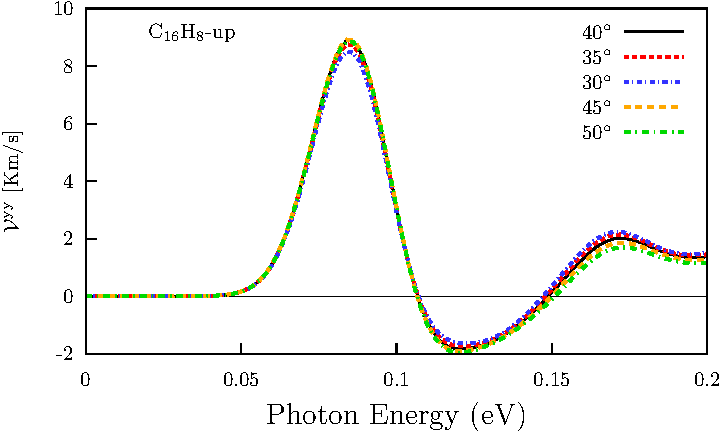
\includegraphics[width=0.45\textwidth]{upplots/up-vab-yy-angcomp.pdf}\\
    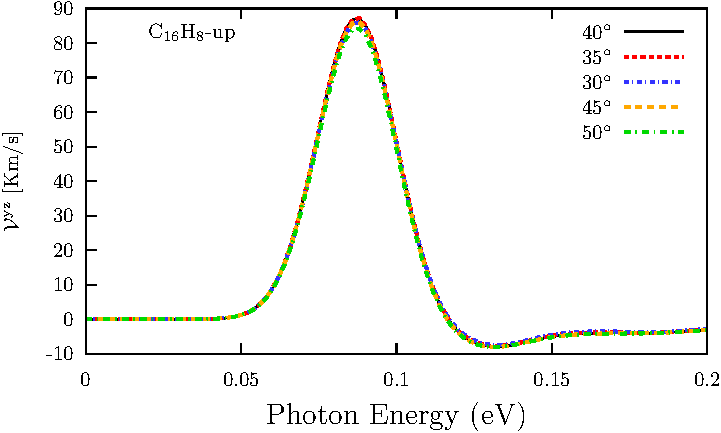
\includegraphics[width=0.45\textwidth]{upplots/up-vab-yz-angcomp.pdf}
    \caption{Cheking angle of incidence for $yb$ components.}
    \label{fig:up-ybangcomp}
\end{figure}
\begin{figure}[ht]
    \centering
    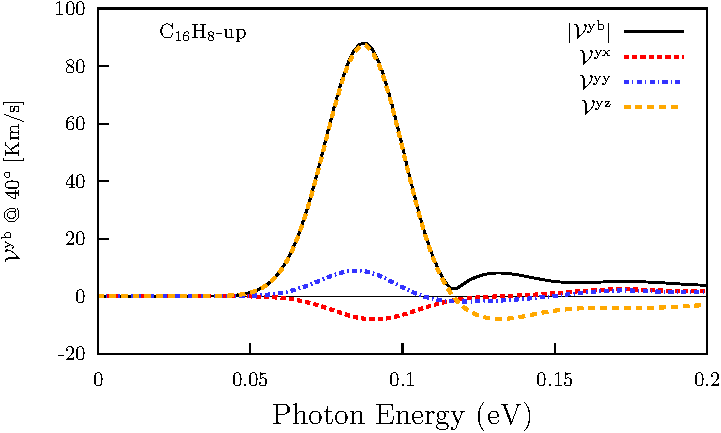
\includegraphics[width=0.7\textwidth]{upplots/up-vab-yb-1.pdf}
    \caption{Three components of $\mathcal{V}^{\mathrm{yb}} $ @ 40$^{\circ}$.}
    \label{fig:up-vyb1}
\end{figure}


%%%%%%%%%%%%%%%%%%%%%%%%%%%%% xb [1.8:2.1] %%%%%%%%%%%%%%%%%%%%%%%%%%%%%%%%%%%%%

\subsection{$\mathcal{V}^{\mathrm{xb}} $: energy range: 1.8--2.1 eV }


\begin{figure}[h]
    \centering
    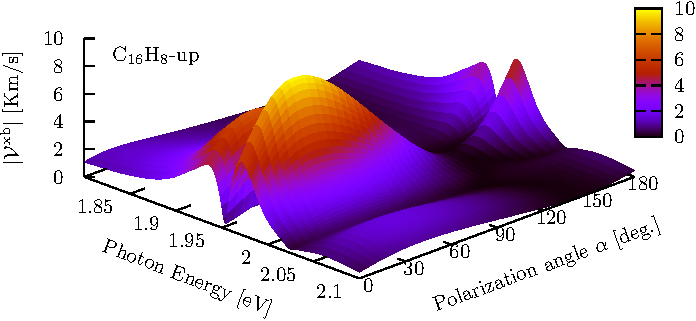
\includegraphics[width=0.7\textwidth]{upplots/up-magvxb-incang-2-4545.pdf}
    \caption{The most intense response for $\mathcal{V}^{\mathrm{xb}} $ is for 
    40$^{\circ}$.}
    \label{fig:up-magxbincang2}
\end{figure}
\begin{figure}[h]
    \centering
    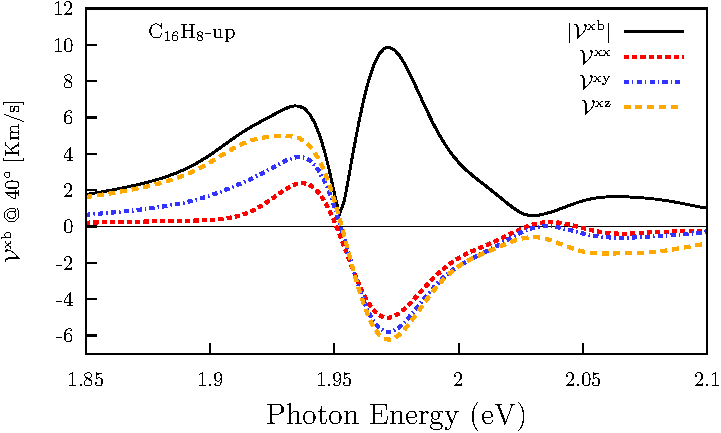
\includegraphics[width=0.7\textwidth]{upplots/up-vab-xb-2.pdf}
    \caption{Three components of $\mathcal{V}^{\mathrm{xb}} $ @ 40$^{\circ}$.}
    \label{fig:up-vxb2}
\end{figure}


\begin{figure}[ht]
    \centering
    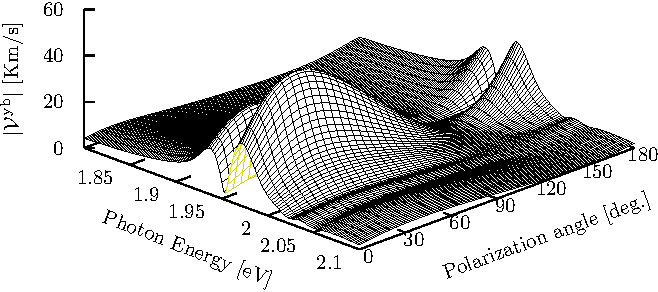
\includegraphics[width=0.7\textwidth]{upplots/up-magvyb-incang-2-4545.pdf}
    \caption{The most intense response for $\mathcal{V}^{\mathrm{yb}} $ is for 
    40$^{\circ}$.}
    \label{fig:up-magybincang2}
\end{figure}
\begin{figure}[ht]
    \centering
    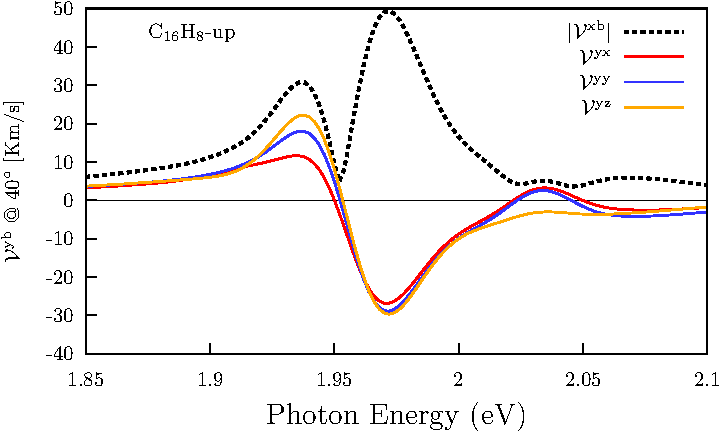
\includegraphics[width=0.7\textwidth]{upplots/up-vab-yb-2.pdf}
    \caption{Three components of $\mathcal{V}^{\mathrm{yb}} $ @ 40$^{\circ}$.}
    \label{fig:upvyb2}
\end{figure}

\clearpage

%%%%%%%%%%%%%%%%%%%%% |V^{ab}| [0.0:0.2] rtp comp %%%%%%%%%%%%%%%%%%%%%%%%%%%%%%
\subsection{$|\mathcal{V}^{\mathrm{ab}}|$ energy range 0.0--0.2 eV: angles
$\theta$ and $\varphi$, layers, and comparison with CdSe and GaAs}

\begin{figure}[ht]
    \centering
    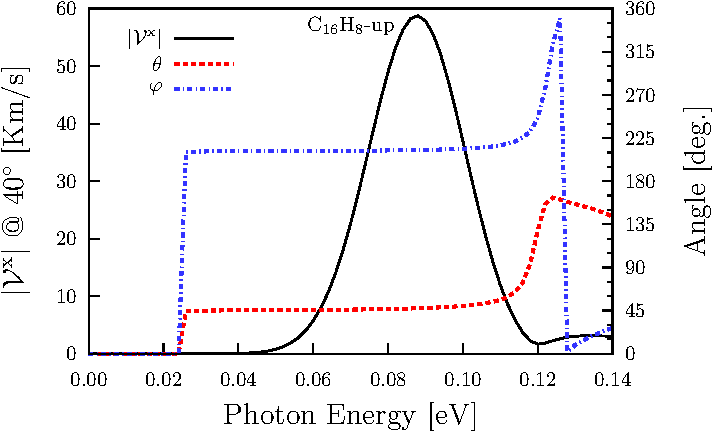
\includegraphics[width=0.7\textwidth]{upplots/up-vxb-rtp-1.pdf}
    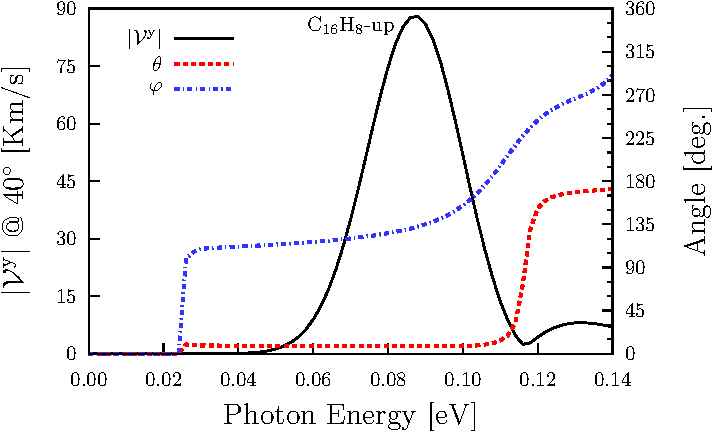
\includegraphics[width=0.7\textwidth]{upplots/up-vyb-rtp-1.pdf}
    \caption{$|\mathcal{V}^{\mathrm{ab}}|$ (solid line, leftside scale) and the
    corresponding angles $\theta$ and $\varphi$ (dashed lines, rightside scale).}
    \label{fig:up-rtp1}
\end{figure}

\begin{figure}[ht]
    \centering
    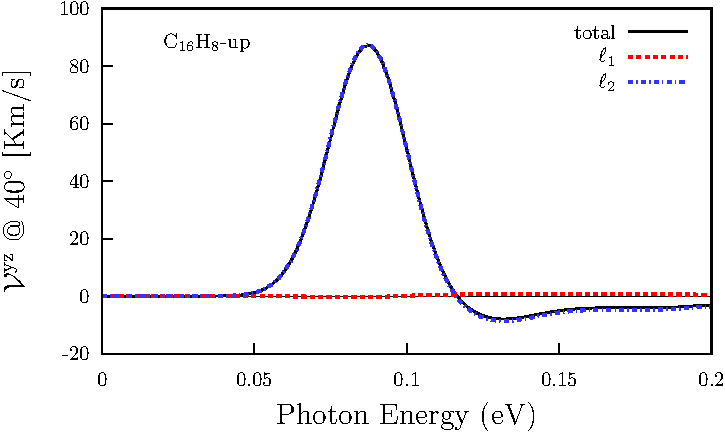
\includegraphics[width=0.7\textwidth]{upplots/up-vyz-layers-1.pdf}
    \caption{Layer decomposition for the most intense response:
    $\mathcal{V}^{\mathrm{yz}}$.}
    \label{fig:up-lay1}
\end{figure}

\begin{figure}[ht]
    \centering
    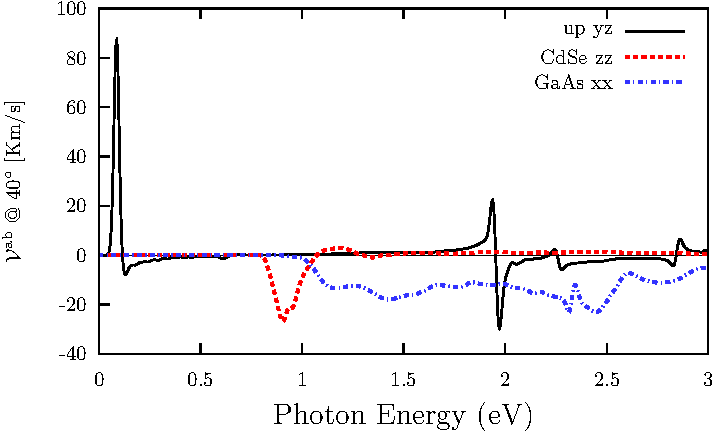
\includegraphics[width=0.7\textwidth]{upplots/up-vab-yz-comp-1.pdf}
    \caption{Comparisson of the most intense response vs the most intense
    responses of CdSe and GaAs.}
    \label{fig:up-comp1}
\end{figure}

%%%%%%%%%%%%%%%%%%%%% |V^{ab}| [1.8:2.1] rtp comp %%%%%%%%%%%%%%%%%%%%%%%%%%%%%%
\subsection{$|\mathcal{V}^{\mathrm{ab}}|$, angles
$\theta$ and $\varphi$, layers, and comparison with CdSe and GaAs for the energy
range of 1.8--2.1 eV}

\begin{figure}[ht]
    \centering
    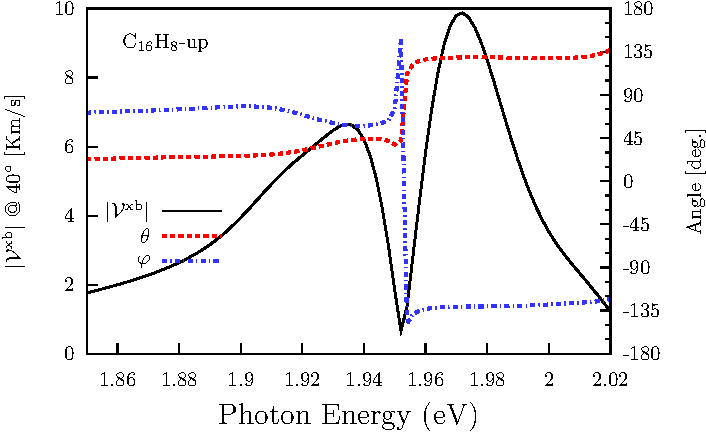
\includegraphics[width=0.7\textwidth]{upplots/up-vxb-rtp-2.pdf}
    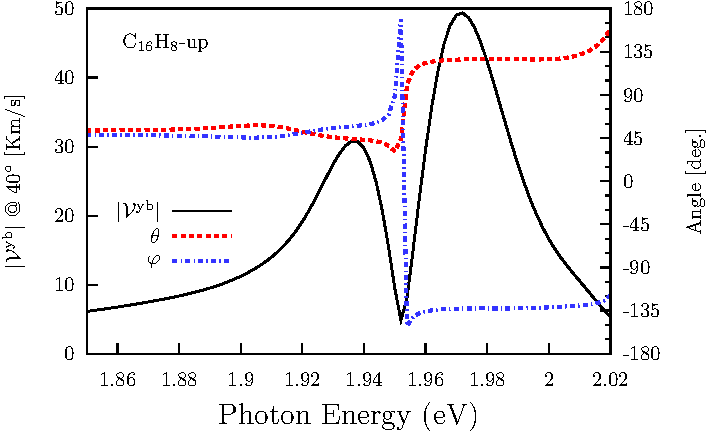
\includegraphics[width=0.7\textwidth]{upplots/up-vyb-rtp-2.pdf}
    \caption{$|\mathcal{V}^{\mathrm{ab}}|$ (solid line, leftside scale) and the
    corresponding angles $\theta$ and $\varphi$ (dashed lines, rightside scale).}
    \label{fig:up-rtp2}
\end{figure}

\begin{figure}[ht]
    \centering
    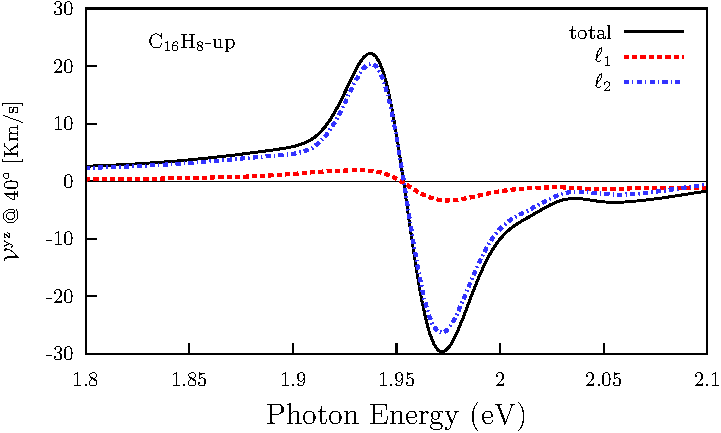
\includegraphics[width=0.7\textwidth]{upplots/up-vyz-layers-2.pdf}
    \caption{Layer decomposition for the most intense response:
    $\mathcal{V}^{\mathrm{yz}}$.}
    \label{fig:up-lay2}
\end{figure}

\begin{figure}[ht]
    \centering
    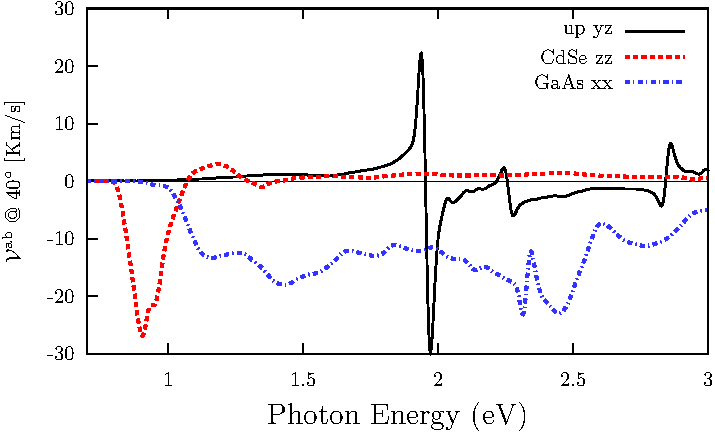
\includegraphics[width=0.7\textwidth]{upplots/up-vab-yz-comp-2.pdf}
    \caption{Comparisson of the most intense response vs the most intense
    responses of CdSe and GaAs.}
    \label{fig:up-comp2}
\end{figure}

% section up (end)


%%%%%%%%%%%%%%%%%%%%%%%%%%%%%%%%%%%%%%%%%%%%%%%%%%%%%%%%%%%%%%%%%%%%%%%%%%%%%%%%
%%%%%%%%%%%%%%%%%%%%%%%%%%%%%%%%%%% ALT %%%%%%%%%%%%%%%%%%%%%%%%%%%%%%%%%%%%%%%%
%%%%%%%%%%%%%%%%%%%%%%%%%%%%%%%%%%%%%%%%%%%%%%%%%%%%%%%%%%%%%%%%%%%%%%%%%%%%%%%%

\section{alt} % (fold)
\label{sec:alt}

%%%%%%%%%%%%%%%%%%%%%%%%%%%%% xb [0.6:1.0] %%%%%%%%%%%%%%%%%%%%%%%%%%%%%%%%%%%%%
\subsection{$\mathcal{V}^{\mathrm{xb}} $: energy range: 0.6--1.0 eV }
\begin{figure}[h!]
    \centering
    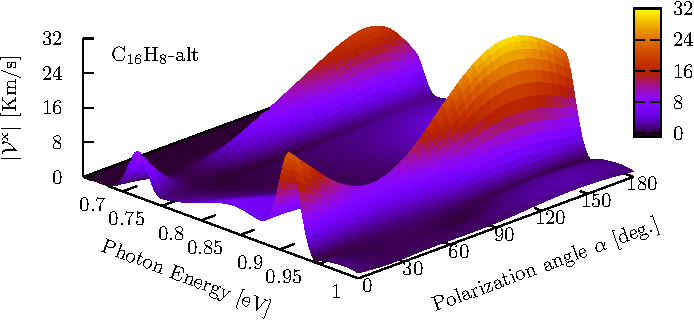
\includegraphics[width=0.7\textwidth]{altplots/alt-magvxb-incang-4545.pdf}
    \caption{The most intense response for $\mathcal{V}^{\mathrm{xb}} $ is for 
    145$^{\circ}$.}
    \label{fig:alt-magvxbincang1}
\end{figure}
\begin{figure}[h!]
    \centering
    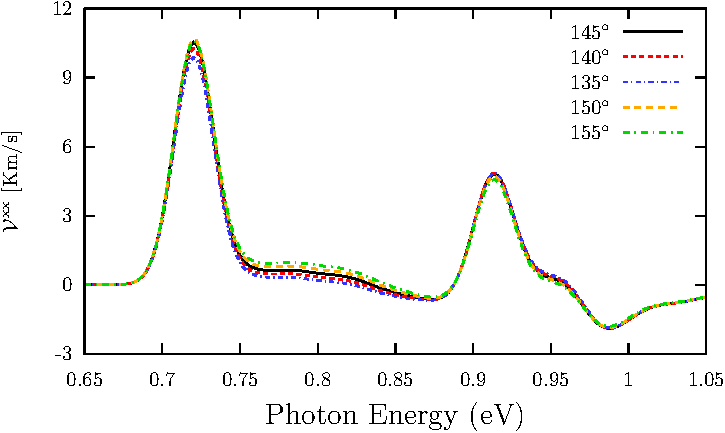
\includegraphics[width=0.45\textwidth]{altplots/alt-vxx.pdf}
    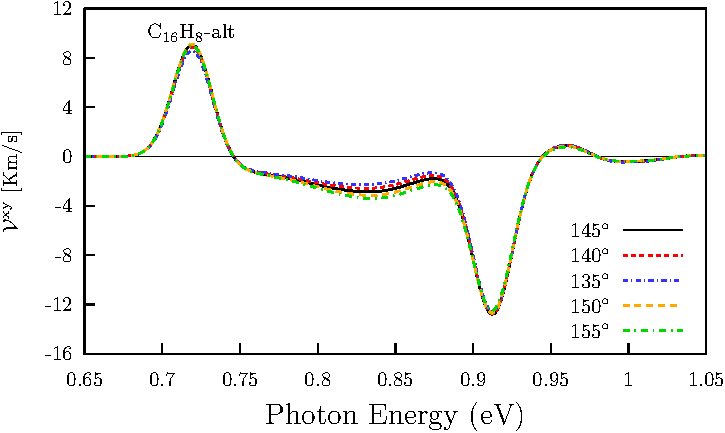
\includegraphics[width=0.45\textwidth]{altplots/alt-vxy.pdf}\\
    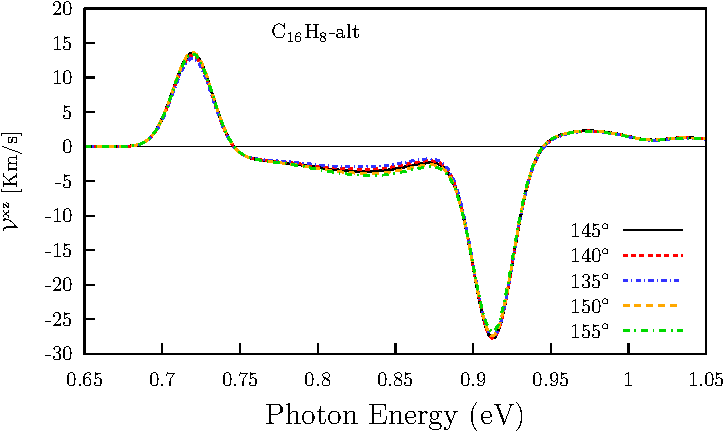
\includegraphics[width=0.45\textwidth]{altplots/alt-vxz.pdf}
    \caption{Cheking angle of incidence for $xb$ components.}
    \label{fig:alt-xbangcomp}
\end{figure}
\begin{figure}[t!]
    \centering
    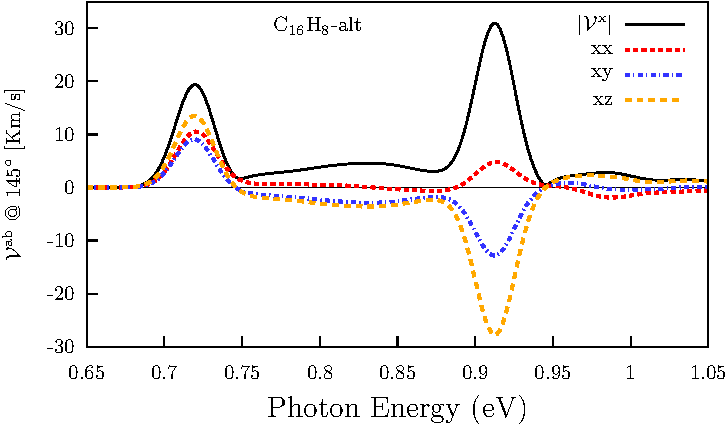
\includegraphics[width=0.7\textwidth]{altplots/alt-vab-xb.pdf}
    \caption{Three components of $\mathcal{V}^{\mathrm{xb}} $ @ 145$^{\circ}$.}
    \label{fig:alt-vxb1}
\end{figure}


%%%%%%%%%%%%%%%%%%%%%%%%%%%%% yb [0.6:1.0] %%%%%%%%%%%%%%%%%%%%%%%%%%%%%%%%%%%%%
\subsection{$\mathcal{V}^{\mathrm{yb}} $: energy range: 0.6--1.0 eV }
\begin{figure}[h]
    \centering
    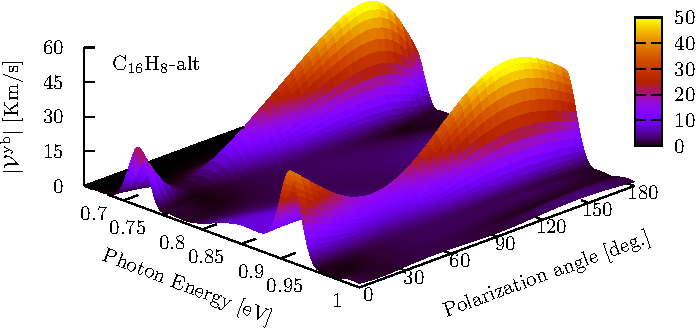
\includegraphics[width=0.7\textwidth]{altplots/alt-magvyb-incang-4545.pdf}
    \caption{The most intense response for $\mathcal{V}^{\mathrm{yb}} $ is for 
    145$^{\circ}$.}
    \label{fig:alt-magvybincang1}
\end{figure}
\begin{figure}[ht]
    \centering
    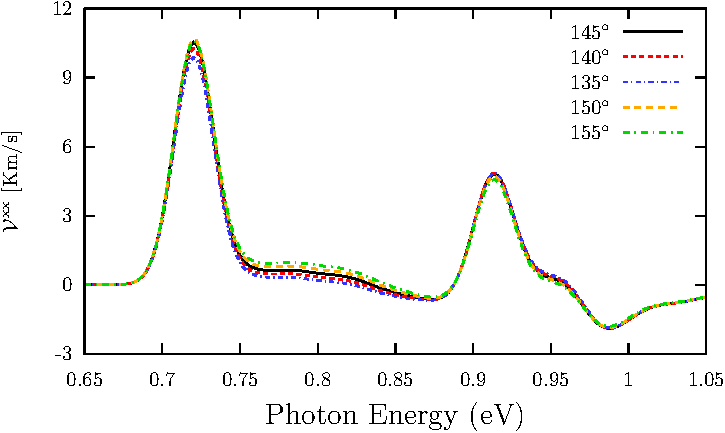
\includegraphics[width=0.45\textwidth]{altplots/alt-vxx.pdf}
    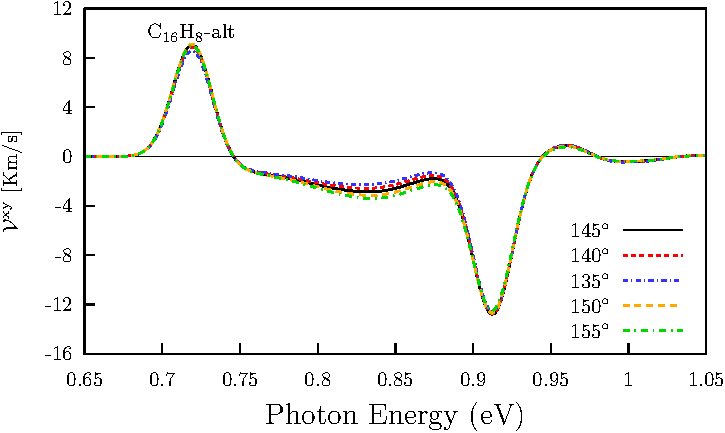
\includegraphics[width=0.45\textwidth]{altplots/alt-vxy.pdf}\\
    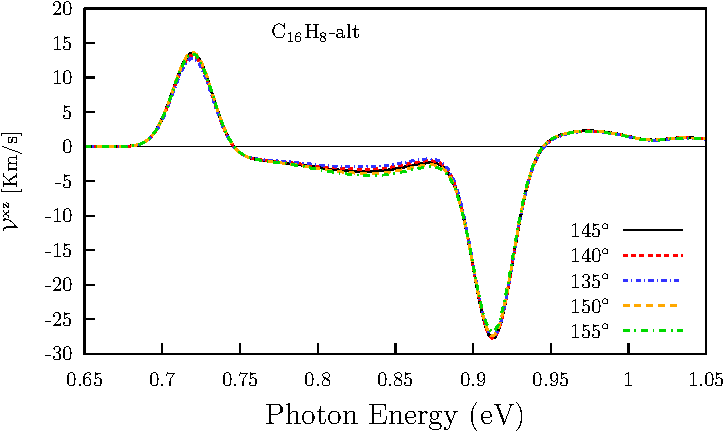
\includegraphics[width=0.45\textwidth]{altplots/alt-vxz.pdf}
    \caption{Cheking angle of incidence for $yb$ components.}
    \label{fig:alt-ybangcomp}
\end{figure}
\begin{figure}[ht]
    \centering
    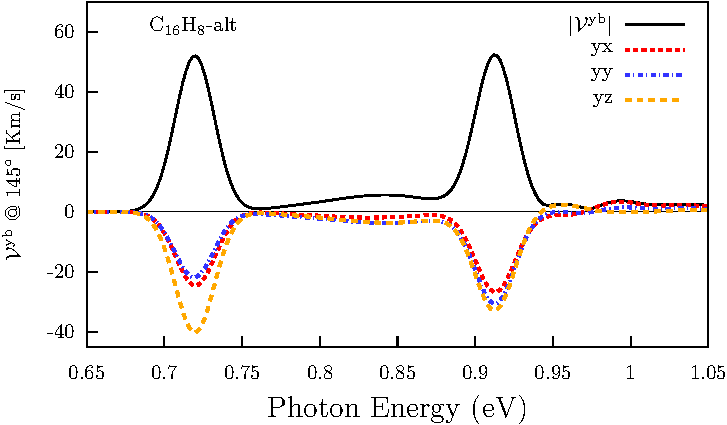
\includegraphics[width=0.7\textwidth]{altplots/alt-vab-yb.pdf}
    \caption{Three components of $\mathcal{V}^{\mathrm{yb}} $ @ 145$^{\circ}$.}
    \label{fig:alt-vyb1}
\end{figure}

%%%%%%%%%%%%%%%%%%%%% |V^{ab}| [0.6:1.0] rtp comp %%%%%%%%%%%%%%%%%%%%%%%%%%%%%%
\subsection{$|\mathcal{V}^{\mathrm{ab}}|$, angles
$\theta$ and $\varphi$, layers, and comparison with CdSe and GaAs.}
\begin{figure}[ht]
    \centering
    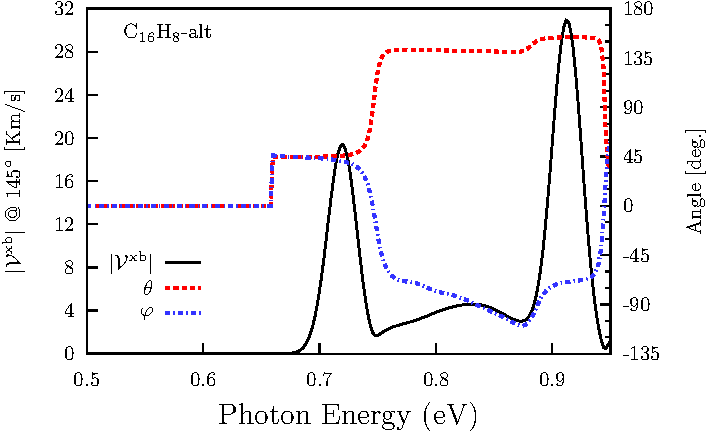
\includegraphics[width=0.7\textwidth]{altplots/alt-vxb-rtp.pdf}
    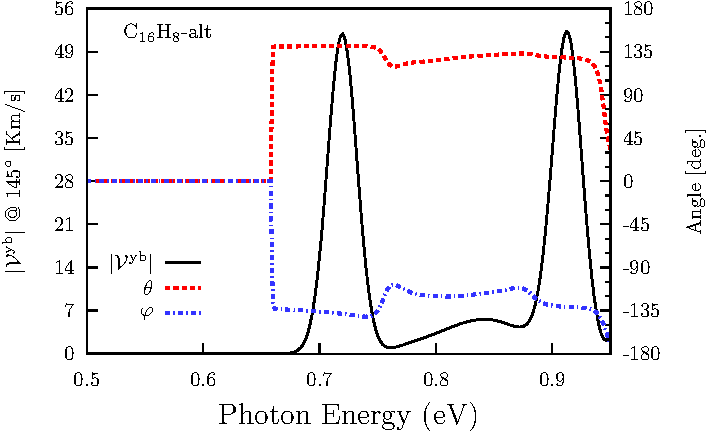
\includegraphics[width=0.7\textwidth]{altplots/alt-vyb-rtp.pdf}
    \caption{$|\mathcal{V}^{\mathrm{ab}}|$ (solid line, leftside scale) and the
    corresponding angles $\theta$ and $\varphi$ (dashed lines, rightside scale).}
    \label{fig:alt-rtp}
\end{figure}

\begin{figure}[ht]
    \centering
    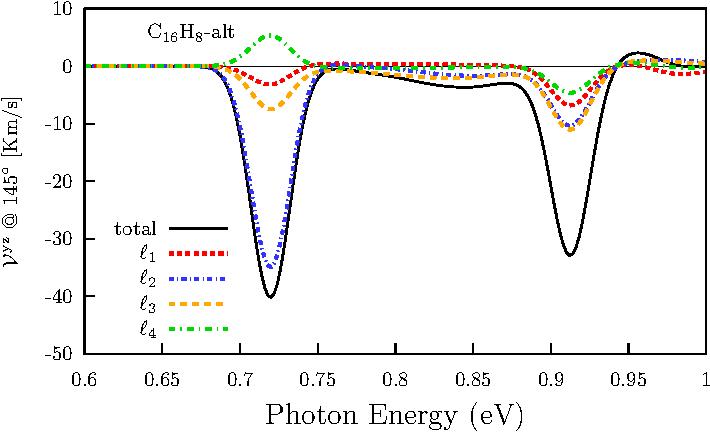
\includegraphics[width=0.7\textwidth]{altplots/alt-vyz-layers.pdf}
    \caption{Layer decomposition for the most intense response:
    $\mathcal{V}^{\mathrm{yz}}$.}
    \label{fig:alt-lay}
\end{figure}

\begin{figure}[ht]
    \centering
    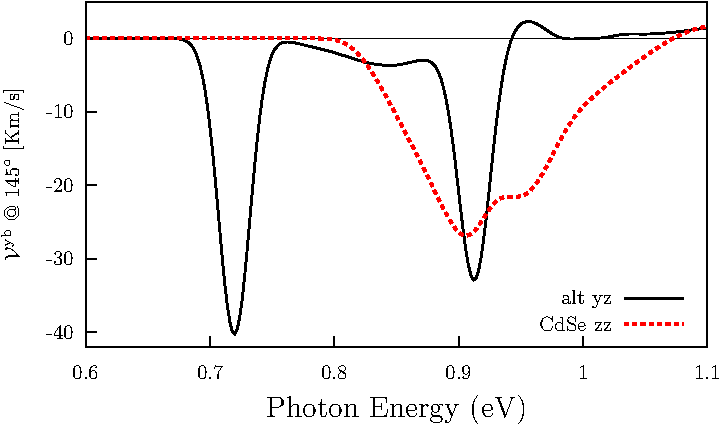
\includegraphics[width=0.7\textwidth]{altplots/alt-vab-comp.pdf}
    \caption{Comparisson of the most intense response vs the most intense
    responses of CdSe and GaAs.}
    \label{fig:alt-comp}
\end{figure}



% section alt (end)




\end{document}
